\documentclass[11pt]{article}

%\usepackage{amsmath, amssymb, fullpage, amsthm, array, algorithm2e,graphicx}
\usepackage{graphicx}
\usepackage{url}
\usepackage[colorlinks=true, citecolor=blue, linkcolor=blue]{hyperref}

\graphicspath{{images/}}

\setlength{\oddsidemargin}{0in}
\setlength{\evensidemargin}{0in}
\setlength{\textwidth}{6.5in}
%\setlength{\topmargin}{-0.4in}
\setlength{\textheight}{8in}


\title{Designing Turk Experiments for Visual Statistical Inference}
\author{Mahbubul Majumder, Heike Hofmann, Dianne Cook\\
        Department of Statistics, Iowa State University}


\begin{document}

\tableofcontents

\maketitle


\begin {abstract} 

Human observers are needed to evaluate lineups that are used to test the significance of findings using statistical graphics. One good option is to recruit people from online workplace like Amazon Mechanical Turk (MTurk). It has the facilities to create online task that would allow people to evaluate lineups and get paid. MTurk is designed for simple and easy tasks. The technical design of the underlying experiment for visual inference may be complex and the tools available to design this from MTurk is just too simple. In this paper we present an alternative way to conduct the survey on lineups by designing a separate web application and getting turk worker do their job from this web site. The web site is now hosted and has been in use and multiple experiments were already done. It turns out to be a very efficient way of getting lineups evaluated by online observers. Getting results from this web site is very convenient and secure. This paper also describes how to design MTurk experiments.

\end {abstract}


\section{Introduction} 

There have been some advancements in visual statistical inference since it was first introduced by Buja \cite{buja:2009} where they have proposed formal methods for testing the significance of findings using lineup protocols. In visual statistical inference the test statistics is a plot of the observed data. This plot is placed randomly in a layout of plots called lineup. The rest of the plots in the lineups are generated from the model specified by the null hypothesis. A human observer is then asked to evaluate the lineup. If the observer detects the actual plot in the lineup, the null hypothesis is rejected.

The power of visual test is studied by Majumder \cite{majumder:2013} and it is revealed that power could be as good as conventional test and some times even better. But where the conventional test does not exists, visual inference could be the only inferential procedure without compromising a lot in power. 

These developments open up a whole new area of statistical research where lineups need to be evaluated by human observer. There are some reasons a researcher needs to evaluate lineups. One is to assess the power of the visual test \cite{heike:2012} for different visual test statistics. The another reason would be to make decision based on the lineup, i.e., to use lineup protocol in practical application \cite{niladri:2012}. Other reasons could be to present the results of the conventional test with visual tools such as lineup.  



%The effect of different graphical design while selecting visual test statistic is studied by Heike \cite{heike:2012}.

The power of visual test can be obtained theoretically \cite{majumder:2013} under some conditions. In general it is hard to obtain explicitly with a mathematical formula since it is very much dependent on individual observation. One approach to estimate the power is to recruit observers to evaluate lineups obtained in known controlled situation \cite{majumder:2013}. It is better to get observers as diverse as possible without being much concerned about the observers' formal training about statistical graphics.



\subsection{Amazon Mechanical Turk (MTurk)}

Amazon Mechanical Turk web site \cite{turk} is a very good resource for recruiting reliable survey participants for visual experiments. This is the place where people come to work online and get paid. The web site is very convenient and reliable to collect simple experiment data. But to design a complex experiment like what we need using their web interface is a pain and often a very time consuming work. So, to run the turk experiment we felt the necessity for a well customized web site where the lineups presented to the observers could be easily controlled according to the experimental design. The work flow design of such a mechanism is shown in figure \ref{fig:turk_work_flow}. The plan is to forward turk workers to a well customized web site while payment could be processed from turk web site. This facilitates getting data directly in a local server.

Figure \ref{fig:amazon_task} displays an example of such a task taken from their web site. In this task a worker just has to select from a pool of options and submit the task. The instructions are usually accompany the task and they are very simple and easy to follow. 

\begin{figure}[htbp] 
   \centering
   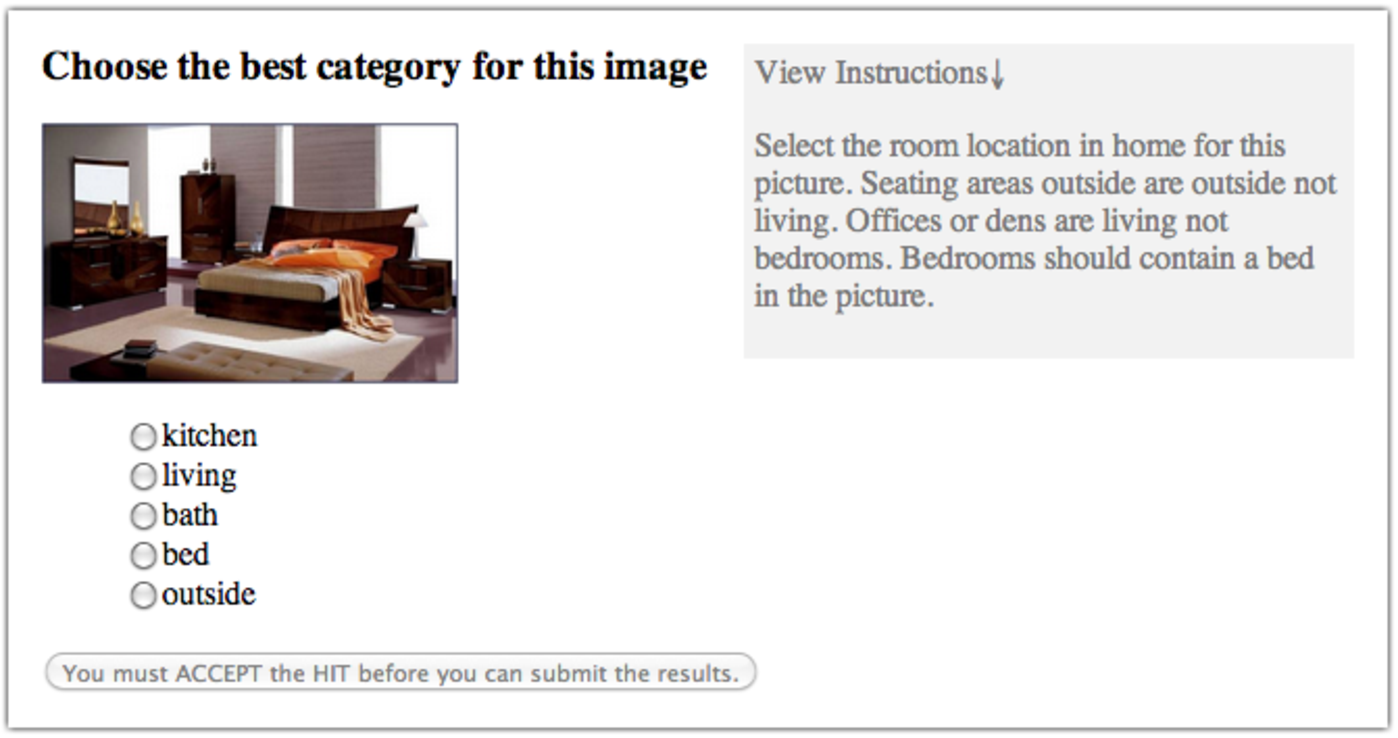
\includegraphics[width=5in]{amazon_task.pdf} 
   \caption{An example of amazon mechanical turk task. Tasks are usually very simple and designed for human evaluations. With each task, simple instructions are given for workers to follow. The workers first accept the task before submitting their response.}
   \label{fig:amazon_task}
\end{figure}


Human observers were recruited to evaluate the experimental lineups through Amazon Mechanical Turk \cite{turk} or MTurk Web site.  It is an online work place where people from around the world can perform some tasks and get paid. Usually tasks are very simple and no specialized training is required. Being a human is the main requirement. Tasks are designed for anyone to do but some tasks may require that workers satisfy some skill level depending on the recruiters need. The tasks are designed such that it does not take much time to complete. Humans are still better than computers in performing these types of tasks. The the amount of money paid for each task is very small as well. 

It is very fast, cheap and reliable to recruit people from MTurk. Thats why it is getting very popular among the researchers who perform human subject experiment. The another benefit is that a very diverse pool of subjects can be recruited which is otherwise very hard to obtain for a study. The researchers can easily filter the workers based on their experimental design, such as recruiting people only from a specific geographical location or a group of people who satisfy certain criteria etc. The recruiter can decide who they pay or not. Workers have to satisfy the task requirement to ensure payment. But at the end it is the recruiter who has the final say. Usually recruiters pay promptly after the task has been done properly and thats why MTurk is very popular among the online job seeker. At any point of time thousands of tasks are available for the thousands of workers around the world. 

Because of its convenience it is getting popular for scientific research study as well. In comparison with a lab study \cite{suri:2010} perform the same study using MTurk and demonstrate that their study results are as good as the lab study results even though MTurk study required less time and cost while provided more convenience. \cite{majumder:2013} recruited people from MTurk for their simulation study in estimating the power of visual statistical inference. They have done numerous pilot studies in lab before doing actual MTurk study and found similar results. \cite{mason:2012} explains various features of MTurk and describes how it can be used as part of human behavioral study.

We designed and developed a web site which enables to display the lineups to the observers as per experimental design. The MTurk workers were redirected to the web site and the data were collected, stored automatically into a local database server. Demographic informations such as age group, gender and education levels were also collected. The time taken for each evaluation is computed based on the time the plot was shown and the time the feedback was received. The location of the observer is determined by the ip address of the observer.

As shown in figure \ref{fig:turk_work_flow} turk workers have to visit the experimental web site and give their consent to participate the survey as per IRB requirement. In the experimental web, there is a option for observers to try some sample lineups to get familiar with the experiment. Once the observers start evaluating the lineups they are sequentially shown a specific number of lineups and at the end they are given a code as a proof for their tusk completion. The payment of the turk worker is processed if they post the code they got from experimental web site. The observers are also asked to provide some demographic information about them to make sure that the code is generated.

\begin{figure}[htbp]
   \centering
       \scalebox{.4}{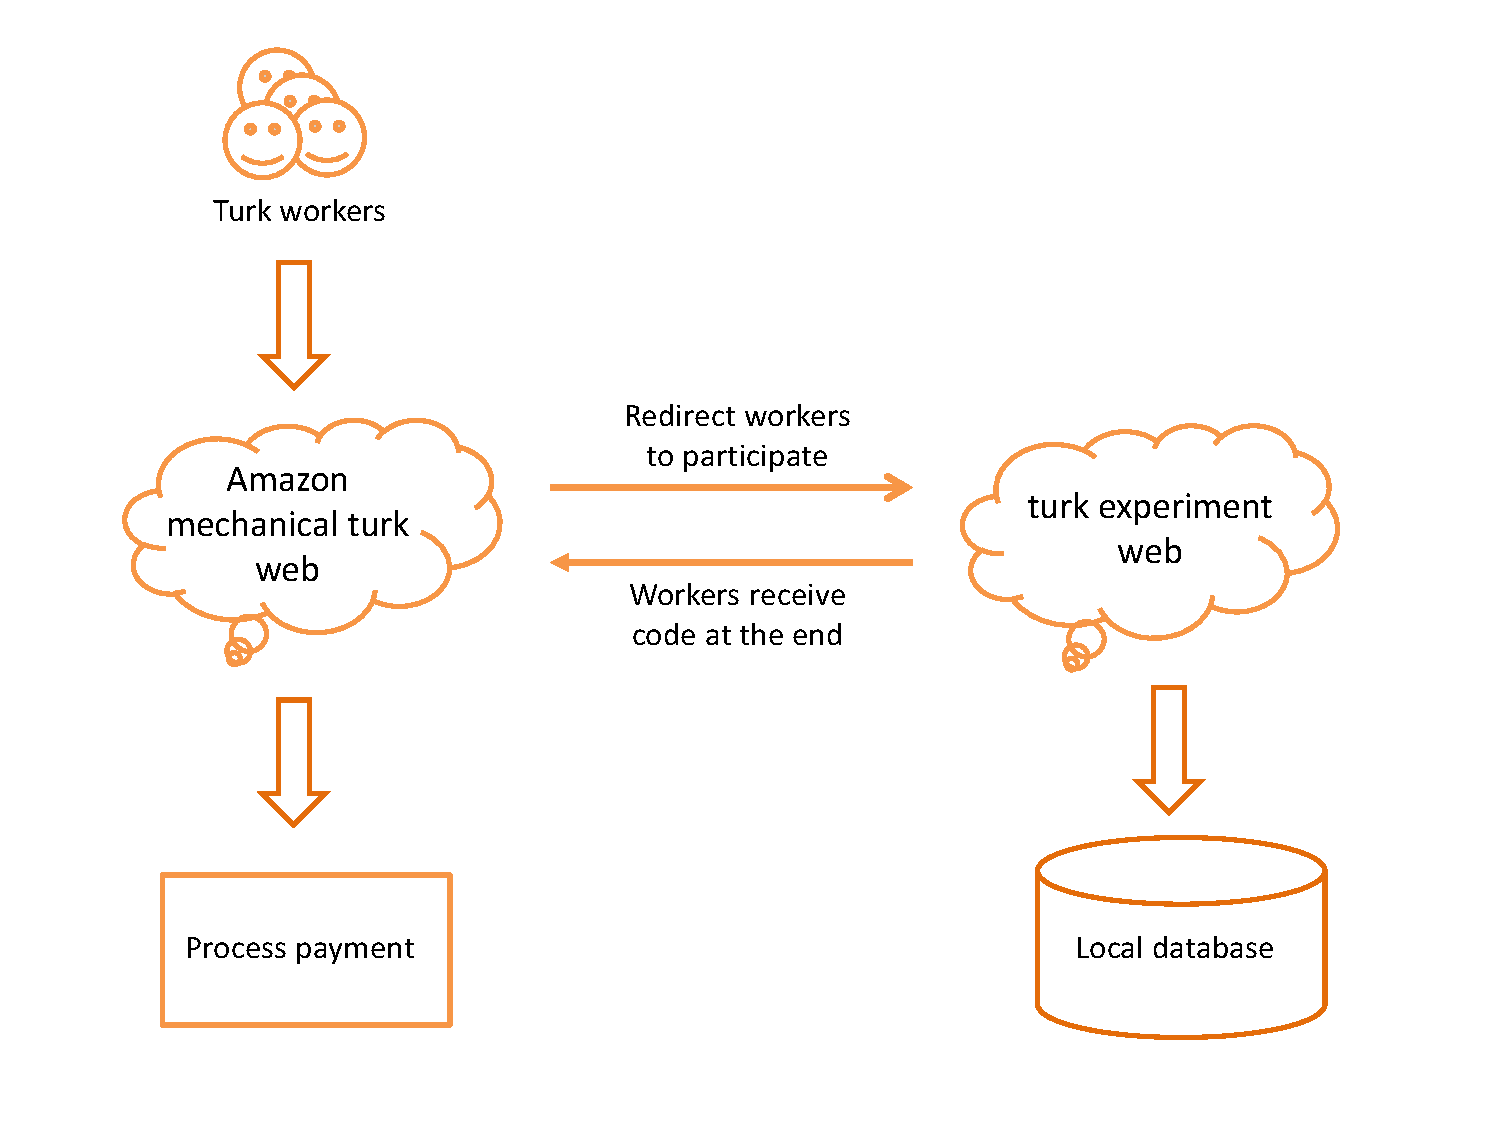
\includegraphics{turk_work_flow.pdf}}
       \caption{Amazon Mechanical Turk workflow and data collection.}
       \label{fig:turk_work_flow}
\end{figure}


\section{Experimental Design} \label{sec:turk_exp}

\subsection{Selecting Parameter of Simulation Experiment} The first consideration for a simulation experiment is to fix the parameters of the model of interest. The very first consideration is the sample size. Other parameters depends on the model of interest. For example we have fixed the parameters in our first Amazon Mechanical Turk experiment as shown in table \ref{tbl:experiment_params}.

\subsection{Sample size estimation} For a given proportion $p$ we want to have margin of error (ME) to be 0.1. Thus we have $$ME =1.96 \sqrt{ \frac 1 n p(1-p)} \le 0.05$$ which gives us the estimation of minimum sample size $$n \geq \frac{p(1-p)}{(0.05/1.96)^2}.$$ Now from the theoretical power curve for each parameter combinations shown in table \ref{tbl:experiment_params} we know the power(say $p$) and thus we can estimate the sample size required for that specific combinations of parameter. We collect data such that each of the parameter combinations in the table \ref{tbl:experiment_params} has approximately the estimated sample size that we calculated here.


\subsection{Procedure to simulate plots for survey} \label{sec:simulate_plot} In the simulation study the very first step is to generate a random sample of data from model of interest for prespecified parameters. We call this data set observed data. While the effect of the natural variability of this data set could be contolled by taking the replication of few samples, it is desirable to study whether we can reduce this variability alternatively. The main reason is to minimize the cost. To make sure that the observed data set truly represents model of interest we are considering three approaches. One is Kolomogorov test statistic approach and the other two approaches are quantiles of p values and closeness of estimated parameters to the true parameters. These three approaches are discussed below.\\

{\bf Kolomogorov test statistic approach:} In this approach we simulate 1000 data sets and obtain Kolmogorov test statistic for each set of data as below. $$D_n=\sup_x |F_n(x)-F(x)|$$ where $F_n(x)=\frac1n \sum_{i=1}^n I_{X_i\le x}$ be the empirical distribution function of fitted residuals, $I_{X_i\le x}$ be the indicator function equal to 1 if $X_i\le x$ and equal to 0 otherwise and $F(x)$ be the cumulative function of normal with mean zero(0) and variance $\sigma^2$. We then keep the data set that has minimum value for Kolmogorov test statistic.  For replication purpose we can generate three observed data sets in similar way.\\

{\bf Quantiles of p-value approach:} With any data set we generate there is a p-value associated with testing $H_0: \beta=0$. In this approach we generate 1000 data sets from the model of interest and obtain p-values associated with $H_0: \beta=0$ for each data set after fitting the same model. Then we construct blocks of p-value such as (0.0-$q_{33}$), ($q_{33}$-$q_{66}$), ($q_{66}$-1) where $q_i$ is the $i$th percentile in the distribution of the p-values. We then randomly select three data sets that have corresponding p-values in the above quantile range. As an example the distribution  of p-values in 1000 simulated data sets for $n$=300, $\beta$=3 and $\sigma$=12 is shown in figure \ref{fig:dist_pvalue}.  Notice that if we like to have three replications of plots, we will have observed data sets with smaller p-values as the distribution is highly right skewed as well as the 33th and 66th percentiles of p-values are 0.0101 and 0.077 respectively. So, another option may be to take the mid points of those quantile ranges and pick the data sets that have those p-values.\\

\begin{figure}[hbtp]
   \centering
       \scalebox{.3}{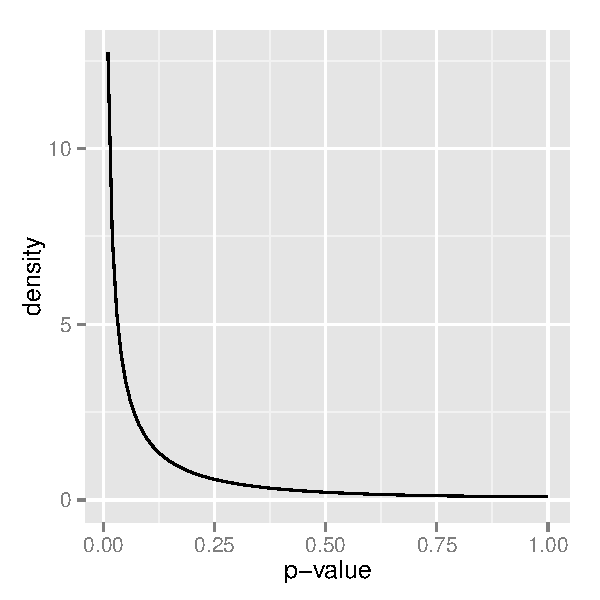
\includegraphics{dist_pvalue.pdf}}
       \caption{Distribution of p-values for $n$=300, $\beta$=3 and $\sigma$=12.}
       \label{fig:dist_pvalue}
\end{figure}

{\bf Closeness of estimated parameters:} When we simulate a data set from the model of interest and again fit the same model with the data set we do not get the parameters estimates same as what we fixed while simulation. It depends on what the standard errors of the parameter estimates are. In our experimental setting we some times have very different estimates for small parameter values(such as one may get estimated value of 0.5 for true $\beta=3$). In this approach we pick the data set that shows most close estimates of parameters compared to true parameter values.\\

All of these three approaches discussed above has some problems. Kolmogorov method does not necessarily make sure that estimated parameters are close to the true parameters. On the other hand closeness of estimated parameters does not make sure that p value is small enough when we should reject the null hypothesis. Only the quantiles approach seems reasonable as it has much control over p-values and it gives similar data sets that has closest parameter estimates. So we used the quantiles of p-value approach in section \ref{sec:simulate_plot} to obtain three replicated sample of observed data sets for a particular parameter settings.\\

\subsection{Test and Training Lineup} How many test lineup?

How to setup training, randomized or sequential selection of lineup for training.

Example lineup on the homepage should be of size three or four so that more than one lineup can be placed on the homepage.

\subsection{Planing the Turk Task}
Question to ask

Whether reasoning would be collected or not

Multiple or single response

Test plot added or not

Training needed or not

Feedback given after every evaluation or not

How many lineups to show

Are the lineups randomly selected?

 


\section{Web Application for Turk Experiment} We developed a web site to run the Amazon Mechanical Turk experiments.  PHP scripting language is used and embedded with HTML for designing the web site. Javascript is used for validating the input data and producing warning message.  We use  Amazon Mechanical Turk web site to recruit the participants and direct them to our web site to actually participate in the survey. This has allowed us to get the data directly in a secure way from the web and we don't have to depend on the Mechanical Turk web site to transfer data to our server. 

\subsection{Form Design}

\subsection{Database design} The design of the database to store the collected data is shown in Figure \ref{fig:turk_database_design}. It is designed such a way that data from many different experiments can be stored in the same database. In total five separate tables are used. Table turk\_worker contains static information about each turk worker. The location information of each turk worker is stored in ip\_detals table. The information in this table is collected later based on the ip address of each turk worker. Table picture\_delais contains the static information about each lineup. Table feedback is a dynamic table that grows with the number of feedbacks from each turk user. The multiple activities of each turk user are recorded in turk\_activity table. This table also contains the codes provided to the user once they finish the experiment. For our web site we used MySQL database located on a local server.

\begin{figure}[hbtp]
   \centering
       \scalebox{.4}{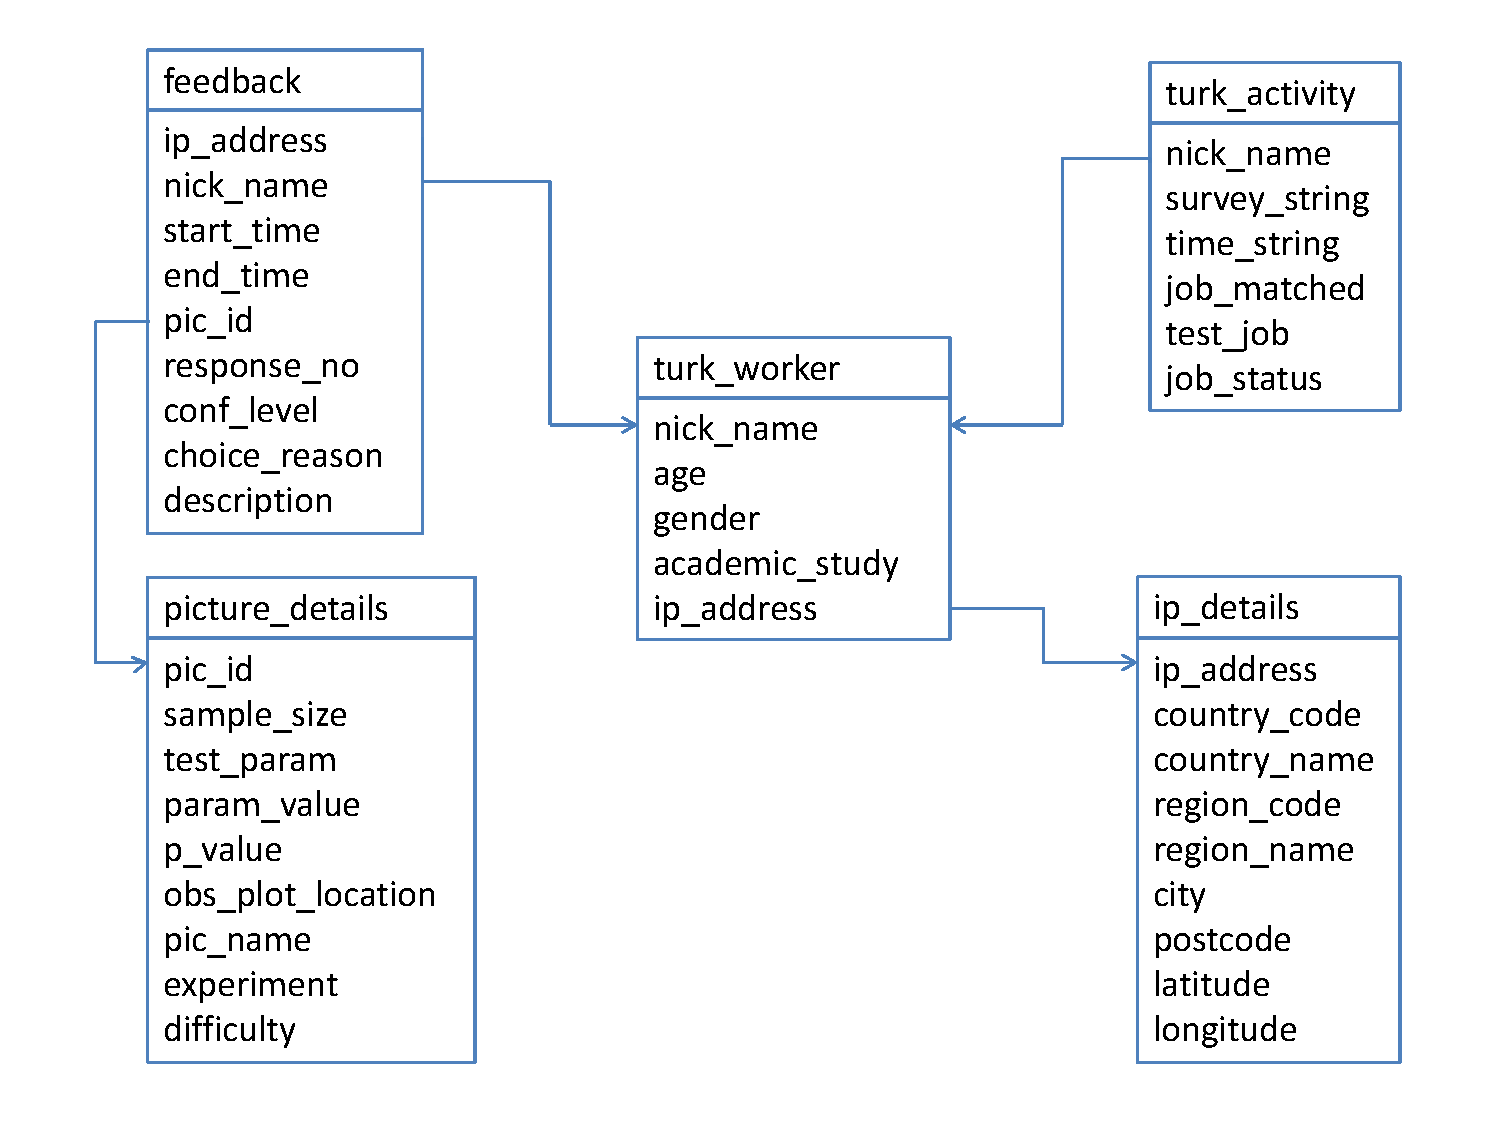
\includegraphics{turk_database_design.pdf}}
       \caption{Database design for Turk experiment data collection. The same database can be used for multiple turk experiments by keeping experiment information in picture details table which contains information about the lineups.}
       \label{fig:turk_database_design}
\end{figure}

\subsection{Data collection} To collect the survey data we developed a web site that shows a plot to an individual and get feedback from that individual. Each individual is asked to provide feedback for at least 10 different plots. The 10 plots that are shown to an individual are randomly chosen with probability proportional to the number of responses required (the sample size) for that plot.

The information collected from each individual is shown in table \ref{tbl:data_info}. Data received from each individual are automatically saved in a secured mysql server maintained by the department of statistics, Iowa state university. 

\begin{table}[hbtp]
\caption{Information Collected from Each Individual}
\centering 
\begin{tabular}{lp{8cm}} 
\hline
Information &  Description \\ %[0.5ex] % inserts table %heading 
\hline
Identification & Nick name or any ID to determine the responses of an Individual \\
Response number & The number of the plot on the lineup plot which the individual thinks the most different than other 19 plots.\\ 
Reason of of choice & Reason why the individual chooses the plot \\
Confidence level & Confidence level of individual choice \\ 
Age group& The age group where the individual belongs \\
Education & The highest level of education completed \\
Gender & Male or female \\
Geographic Location & This information is collected through the ip address of the individual computer \\ 
Time taken & Time taken for each feed back\\
\hline
\end{tabular}
\label{tbl:data_info}
\end{table}	


\subsection{Data collection sequence} Once turk users are directed to our web site, they can see the detailed explanation on how they can perform the task of evaluation. Some simple examples are displayed along with correct responses. The users have options to try some test lineups before going for the actual experiment. But before that they have to provide the informed consent as per IRB requirement. The flow chart for this is shown in Figure \ref{fig:turk_data_flow}

\begin{figure}[hbtp]
   \centering
       \scalebox{.4}{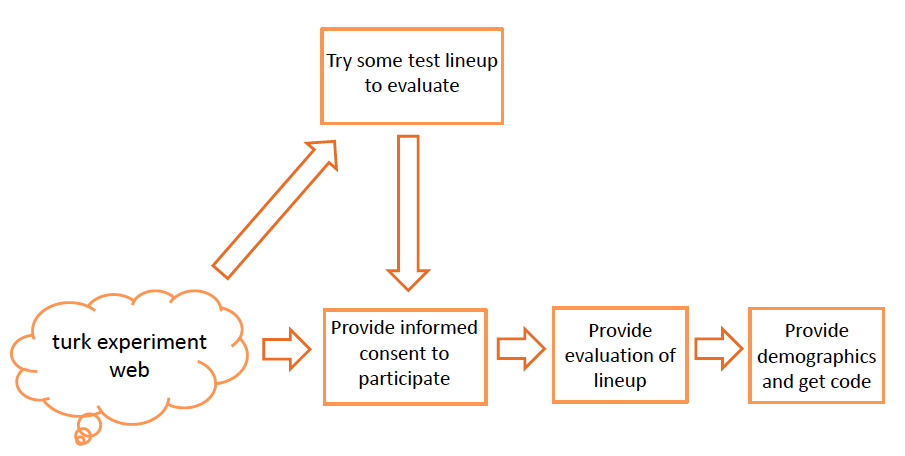
\includegraphics{turk_data_flow.png}}
       \caption{Data collection work flow. Turk worker can try some test lineups before going to the live experiment after providing informed consent.}
       \label{fig:turk_data_flow}
\end{figure}

Two web forms are designed to collect information from the turk users. The first form shown in Figure \ref{fig:turk_web} collects feedback information about a single lineup. The information collected through this form is all about the lineup that includes plot number selected, reasons for selection and the confidence level of the selection. Each turk user is identified by the nick name which is mainly the turk ID. 

Each turk user is shown some specific number of lineups for evaluation. These lineups are randomly selected from a pool of lineups designed for evaluations. The algorithm for how the lineups should be selected to show and what would be the order of display is implemented in the form shown in Figure \ref{fig:turk_web}. Also there is a check for invalid information which is implemented using javascript. If users try to go forward without giving any feedback they are not allowed to do that showing a warning message.

\begin{figure}[hbtp]
   \centering
       \scalebox{.4}{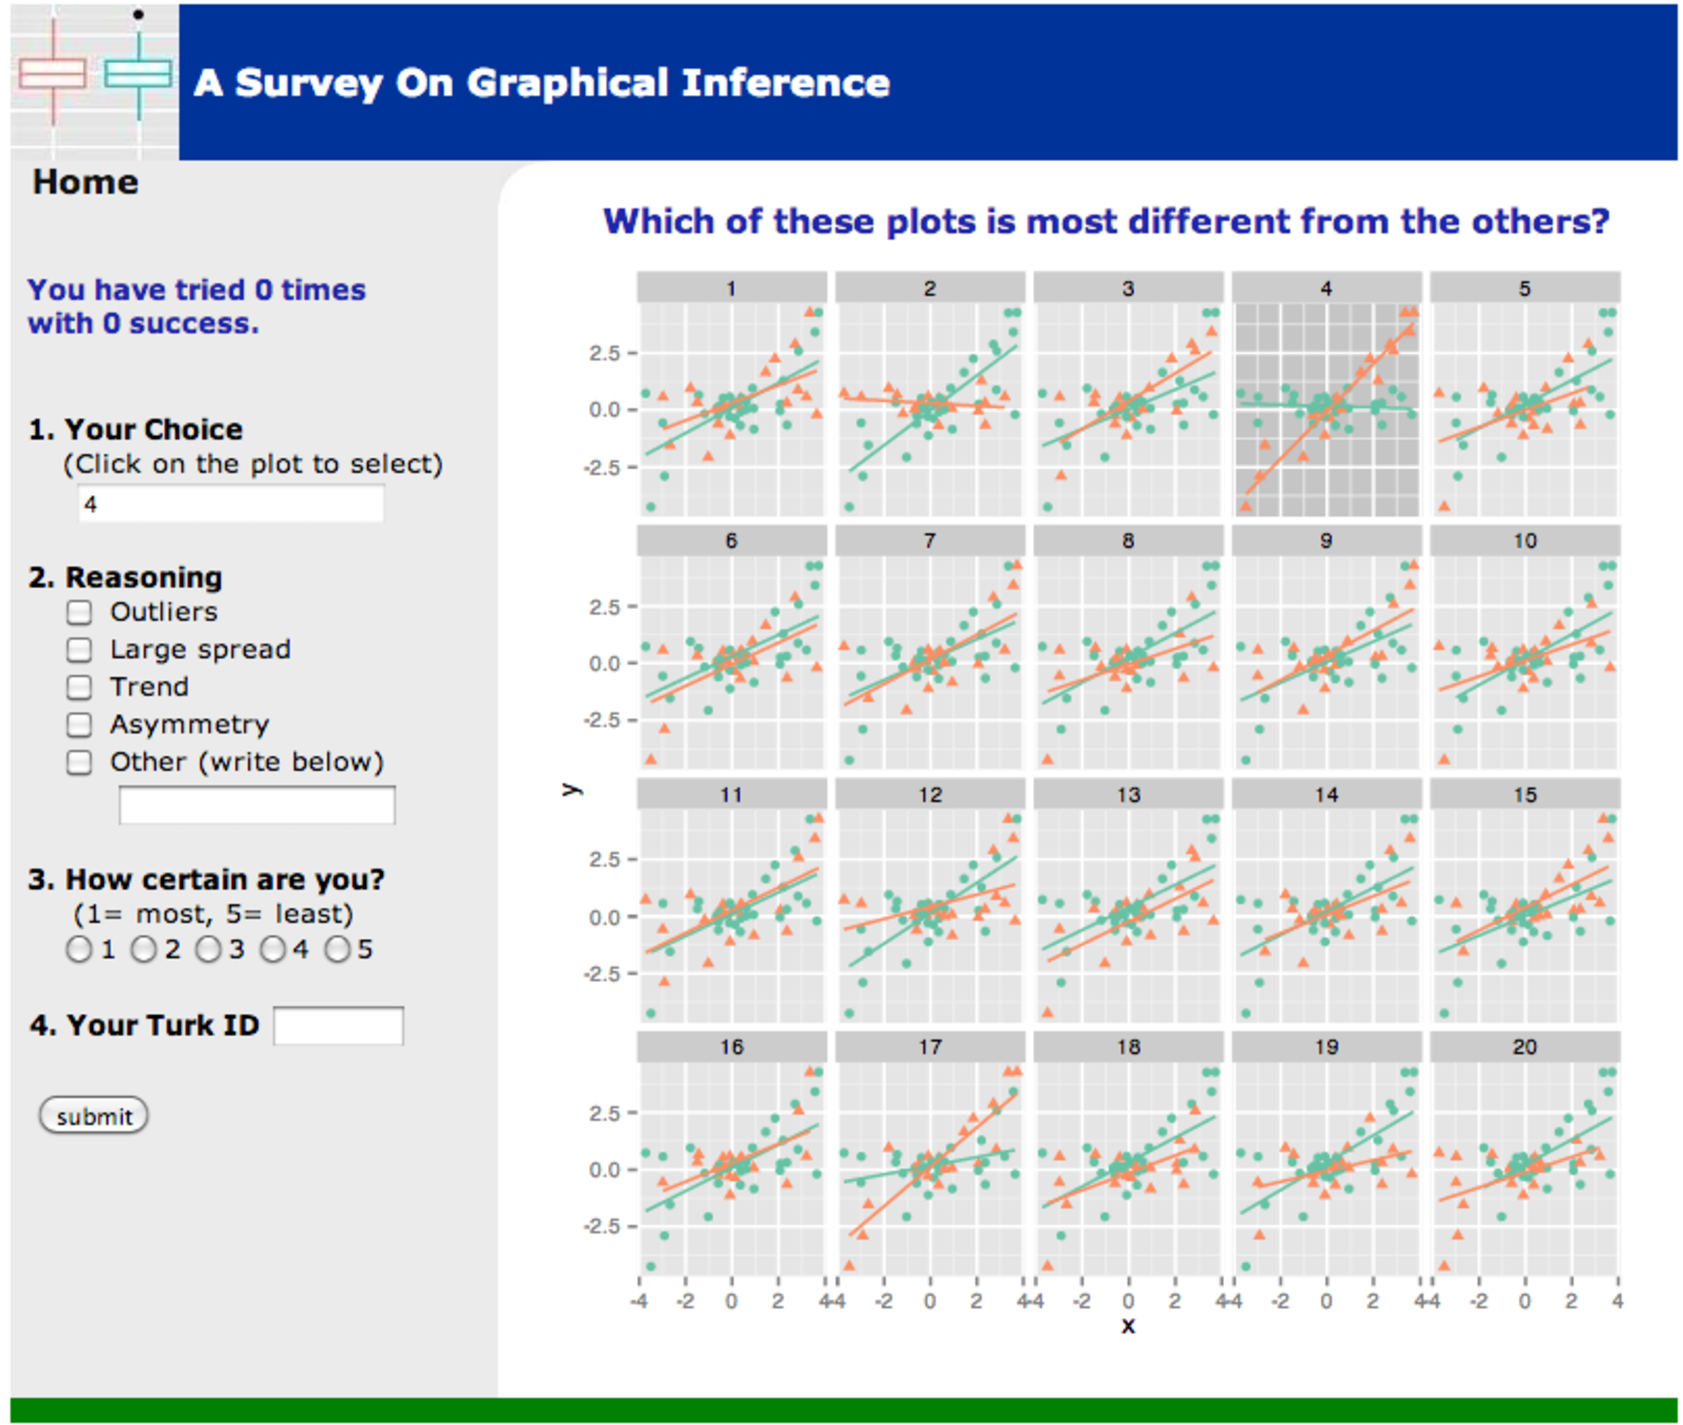
\includegraphics{turk_web.pdf}}
       \caption{A sample data collection form. Lineups are presented at random for evaluations by the turk workers. Scalable Vector Graphics (SVG) is used so that observer can click on the lineup to pick certain plot.}
       \label{fig:turk_web}
\end{figure}

After the evaluation is recorded on a lineup through form shown in Figure \ref{fig:turk_web} another form shown in Figure \ref{fig:turk_web_feedback} is used to give feedback to the turk users whether they correctly identifies the true plot and how many evaluations are recorded from the users. This form is also used to collect demographic and educational information about the user. After the required number of evaluations are obtained from each turk user, a pass code is given as a proof of the completion of the task which then later used for payment purpose.

\begin{figure}[hbtp]
   \centering
       \scalebox{.4}{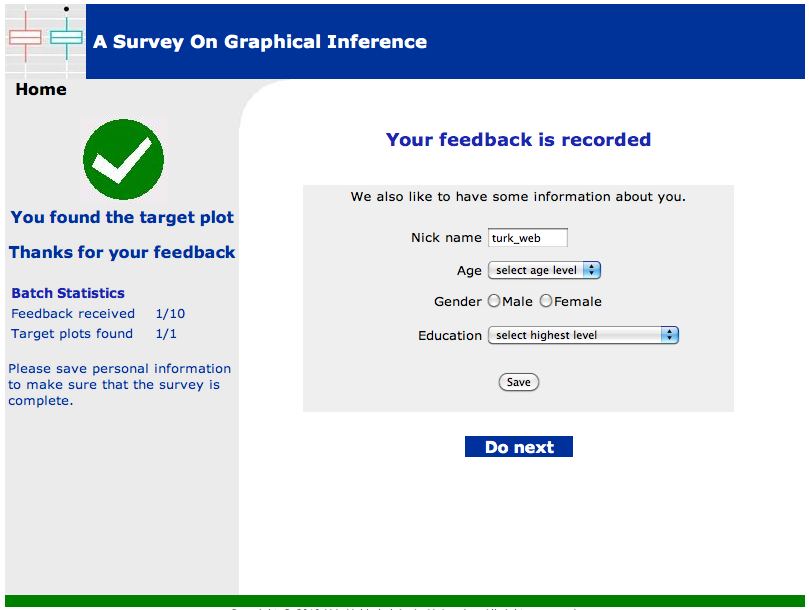
\includegraphics{turk_web_feedback.png}}
       \caption{The turk workers are given feedbacks whether their evaluation for each lineup was correct or not. This works as an incentive for the worker to work more enthusiastically. To ensure the payment, the turk workers have to provide some information using this form.}
       \label{fig:turk_web_feedback}
\end{figure}

\subsection{Data Security and Validity} Consideration to avoid hacking

Check for invalid input

Control for missing imput

\section{Managing Turk Task} Turk workers are usually small payee workers. There several issues related to the payment of their effort. These are briefly discussed in the following section and we intend to work more on this as we progress through this dissertation work. 

\subsection{Creating Task for Lineup Evaluation} Task description, number of people to recruit, time allowed to finish the task, specify the qualification needed, setting the duration of the task, offering the pay per task.

\subsection{Accepting or Rejecting the Task} In our design we keep a test lineup plot which is very easy to evaluate. The general criteria may be to reject payment when workers do not get that easy test lineup plot. Our experience suggest that there are workers who did not get that test plot but their overall success rate is very high. So depending on only one criteria the payment should not be made. These issues would be addressed in our future work based on the several turk experiments that we intend to carry out.

\subsection{Processing Payment}Amazon Mechanical Turk suggest that each worker gets \$6/hour as wage. Thus we need to estimate how much time a tusk may take to complete and based on that we have to specify the payment for each task. Our experience indicates that a better payment lures more serious workers who usually provide cleaner data which is more reliable. We may study this issue while we do multiple turk experiments.

\subsection{Managing Worker} pay bonus, appreciate worker by sending email, block worker etc.

\section{Turk Data Quality}

In this section we intend to analyze the performance of the experiments we did using Amazon Mechanical turk. We have feed back data for the similar plots from both turk workers as well as from the people who regularly participates in the graphics group meeting of our department. We consider later participants as more knowledgeable and trained in seeing pattern in statistical plots. We can use these data to evaluate the performance of the general participants from around the world.



\begin{table}[hbtp]
\caption{Amazon mechanical turk experiments and their properties. Duration in hours per 100 tasks show the popularity of some tasks compared to others.}
\centering
\begin{tabular}{rlrrrrrrr}
  \hline
& Experiment& \multicolumn{2}{c}{ Total Task}& Average & \multicolumn{2}{c}{Duration (hour)} & Payment & Pay rate\\
\cline{3-4} \cline{6-7}
Serial & description & submitted & rejected & time(min) & Actual & 100 task& \$/task & \$/hour\\ 
  \hline
1 & Boxplot & 406 & 106 & 10.68 & 146.48 & 36.08 & 0.50 & 2.81 \\ 
  2 & Scatterplot & 359 &   9 & 10.80 & 42.68 & 11.89 & 1.00 & 5.58 \\ 
  3 & Contaminated plot & 219 &  19 & 13.53 & 126.17 & 57.61 & 1.00 & 2.22 \\ 
  4 & Polar vs Cartesian & 110 &  10 & 20.65 & 11.65 & 10.59 & 1.00 & 2.91 \\ 
  5 & Hist vs density & 234 &  37 & 17.85 & 41.57 & 17.76 & 1.00 & 3.36 \\ 
  6 & Violin vs boxplot & 417 &  17 & 17.95 & 105.87 & 25.39 & 1.00 & 3.34 \\ 
  7 & Group separation & 106 &   6 & 16.13 & 5.15 & 4.86 & 1.00 & 3.72 \\ 
  8 & Sine Illusion & 101 &   1 & 16.52 & 78.38 & 77.60 & 1.00 & 3.63 \\ 
  9 & Gene expression & 103 &   3 & 12.47 & 11.27 & 10.94 & 0.50 & 2.41 \\ 
  10 & Test normality & 406 &   6 & 22.70 & 74.35 & 18.31 & 1.00 & 2.64 \\ 
   \hline
\end{tabular}
\label{tbl:mturk}
\end{table}


\begin{figure}[htbp] 
   \centering
   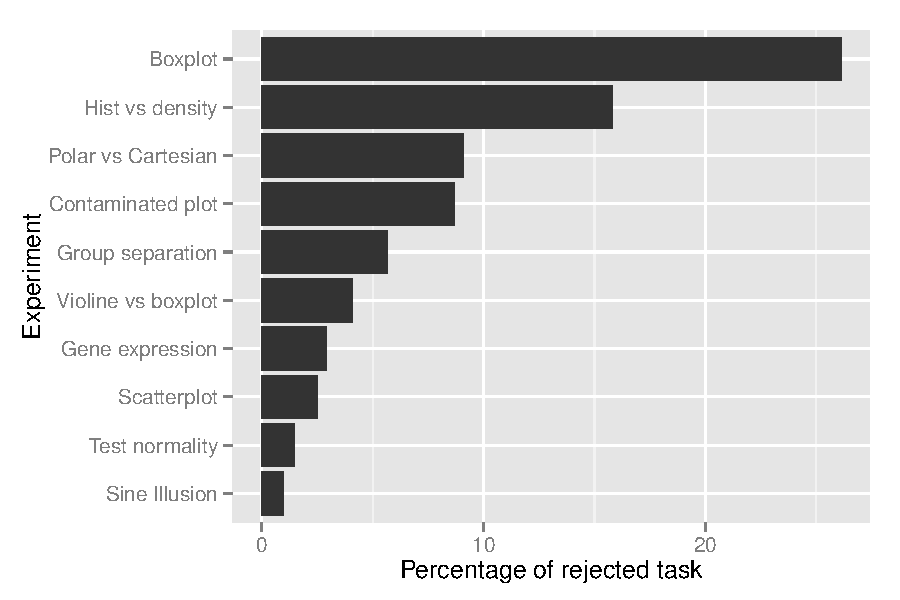
\includegraphics[width=3in]{rejected_task.pdf}
      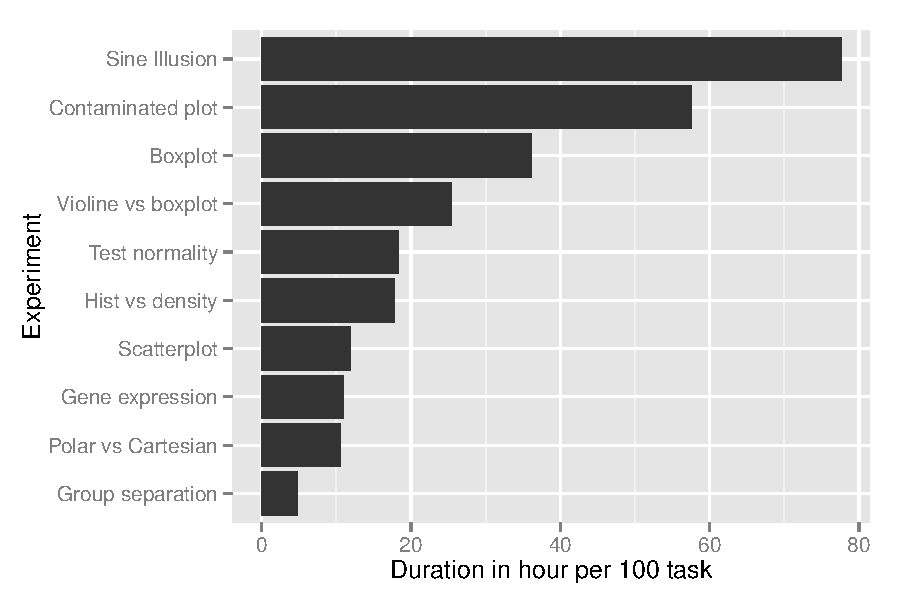
\includegraphics[width=3in]{task_duration.pdf} 
   \caption{Percentage of rejected tasks and duration of each experiment in hour per 100 tasks for each of the 10 experiments. Most of the tasks got rejected for box plot experiment.  Even though the sine illusion experiment took longest to finish the rejection rate is lowest for this experiment.}
   \label{fig:task_duration}
\end{figure}


\subsection{Data Cleaning}

\subsection{Diversity in the Data}

\begin{figure}[hbtp]
   \centering
       \scalebox{.5}{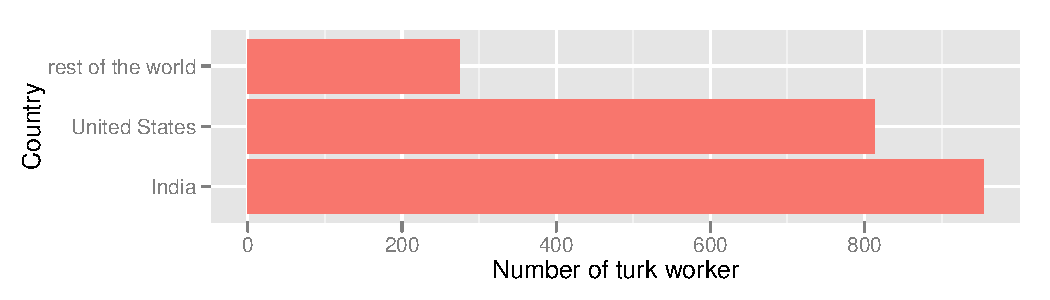
\includegraphics{turker_country.pdf}}
       \scalebox{.5}{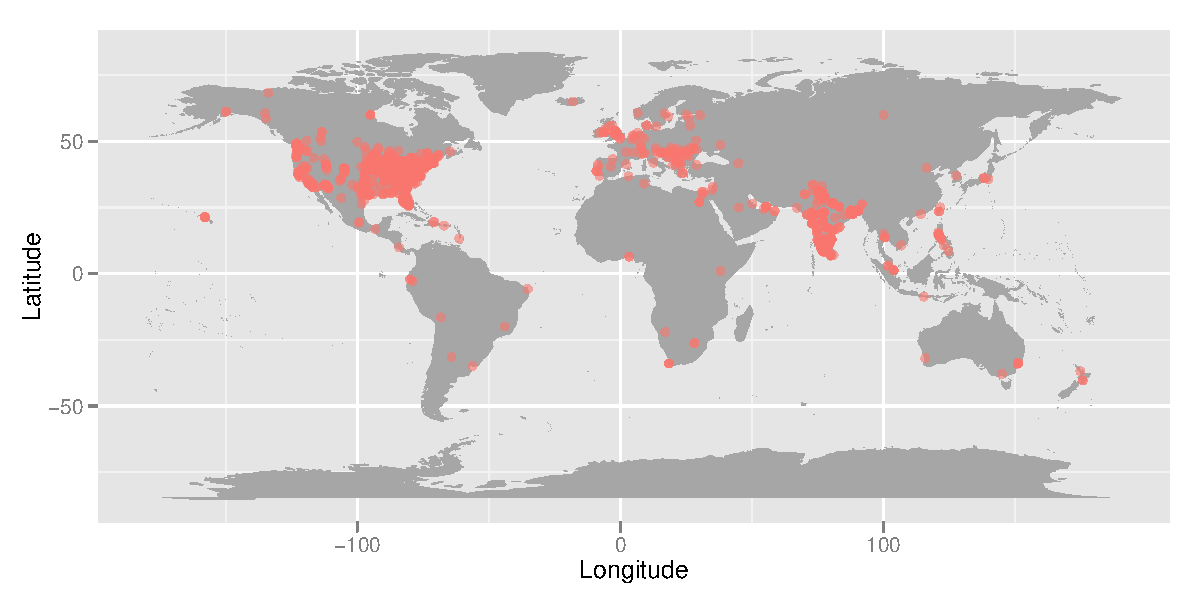
\includegraphics{turker_location.pdf}}       
       \caption{The location of turk workers on the world map shows the geographical diversity of turk workers even though most of the workers come from India and United States.}
       \label{fig:rsq}
\end{figure}

\subsection{Selection Bias} Since data are collected through web interface it is possible to have the selection bias in the turk experiment we did. In this section we intend to analyze to what extent this selection bias has occurred and how we can adjust for this.


Time of the task may recruit from a specific geographical location

Setting up qualification may allow certain workers to do the task

Payment amount may affect the duration of the experiment which may avoid diversity in the geographical locations.


\section{Conclusion} This paper presents a complete solution to the problem of designing a simulation experiment for lineup and recruiting people to get the lineups evaluated. The proposed online application design provides flexibility to control how the multiple lineups would be presented to a observer. It also gives added benefit to record timing of the evaluations. Scalable Vector Graphics (SVG) is used so that observer can click on the lineup to pick certain plot. This also made the multiple plot selection from a lineup easier and convenient. Multiple online experiments are done using this web application and result suggests that the application worked as planned.

The web application is designed such a way that it still produces simple task for the worker who are used to doing so from MTurk. But it gives many flexibilities to the researcher who need lineups to be evaluated as per complex experimental requirement. 



\section{Appendix: What do Turk Workers Pick, $R^2$ or $p$-value?} What do people pick in a lineup plot, p-value or $R^2$? To address this issue we obtain the approximate theoretical relationship between $R^2$ and the power of the classical hypothesis test. Suppose we want to test the significance of the slope ( i.e.,  $H_0: \beta=0$ against $\beta \ne 0$) of a continuous covariate $X$ in  a simple linear regression model setting. Also consider $X \sim N(0,1)$. For a sample of size $n$ this gives us 
\begin{eqnarray*}
Y_i-\bar{Y}& = & \beta_0+\beta_1X_i+\epsilon_i - \beta_0 - \beta_1 \bar{X}- \bar{\epsilon} \\
          & = & \beta_1(X_i-\bar{X})+(\epsilon_i-\bar{\epsilon})
\end{eqnarray*}
Now 
\begin{eqnarray*}
X_i-\bar{X}& = & X_i - \frac1n (X_1 + X_2 + ... + X_i + .....+ X_n) \\
          & = & X_i - \frac1n X_i - \frac1n \sum_{j \neq i}{X_j}\\
          & = & (1-\frac1n)X_i - \frac1n \sum_{j \neq i}{X_j}
\end{eqnarray*}

Thus we have 
\begin{eqnarray*}
E(X_i-\bar{X})^2 & = & (1-\frac1n)EX_i^2 - \left( \frac1n \right )^2 (n-1) EX_j^2 \\
                 & = & (1-\frac1n)^2+ \frac{n-1}{n^2}\\
                 & = & \frac{n-1}{n}
\end{eqnarray*}

Similarly we have 

\begin{eqnarray*}
E(\epsilon_i-\bar{\epsilon})^2 & = & (1-\frac1n)E\epsilon_i^2 - \left( \frac1n \right )^2 (n-1) E\epsilon_j^2 \\
                 & = & \left((1-\frac1n)^2+ \frac{n-1}{n^2} \right) \sigma^2 \\
                 & = & \frac{n-1}{n}\sigma^2
\end{eqnarray*}
Finally we have expected total sum of square (SST) as
\begin{eqnarray*}
E\sum_i{(Y_i-\bar{Y})^2} & = & \sum_i E(Y_i-\bar{Y})^2=\sum_i \left [ \beta_1^2 E(X_i-\bar{X})^2 + E(\epsilon_i-\bar{\epsilon})^2 \right] \\
                 & = & \sum_i\left[ \beta_1^2 \frac{n-1}{n}+  \sigma^2 \frac{n-1}{n}\right]\\
                 & = & (n-1)(\sigma^2+\beta_1^2)
\end{eqnarray*}

We know $E(MSE|X) = \sigma^2$ or $E(SSE/n-2)|X = \sigma^2$ which gives the expected residual or error sum of square as $$E \sum_i (Y_i-\hat Y_i)^2=(n-2)\sigma^2$$
Thus we have the expected regression sum of squares $SSR =  (n-1)(\sigma^2+\beta_1^2) - (n-2)\sigma^2 = (n-1) \beta_1^2+\sigma^2$ This gives $$R^2=\frac{(n-1) \beta_1^2+\sigma^2}{ (n-1)(\sigma^2+\beta_1^2)}$$


\begin{figure}[hbtp]
   \centering
       \scalebox{.3}{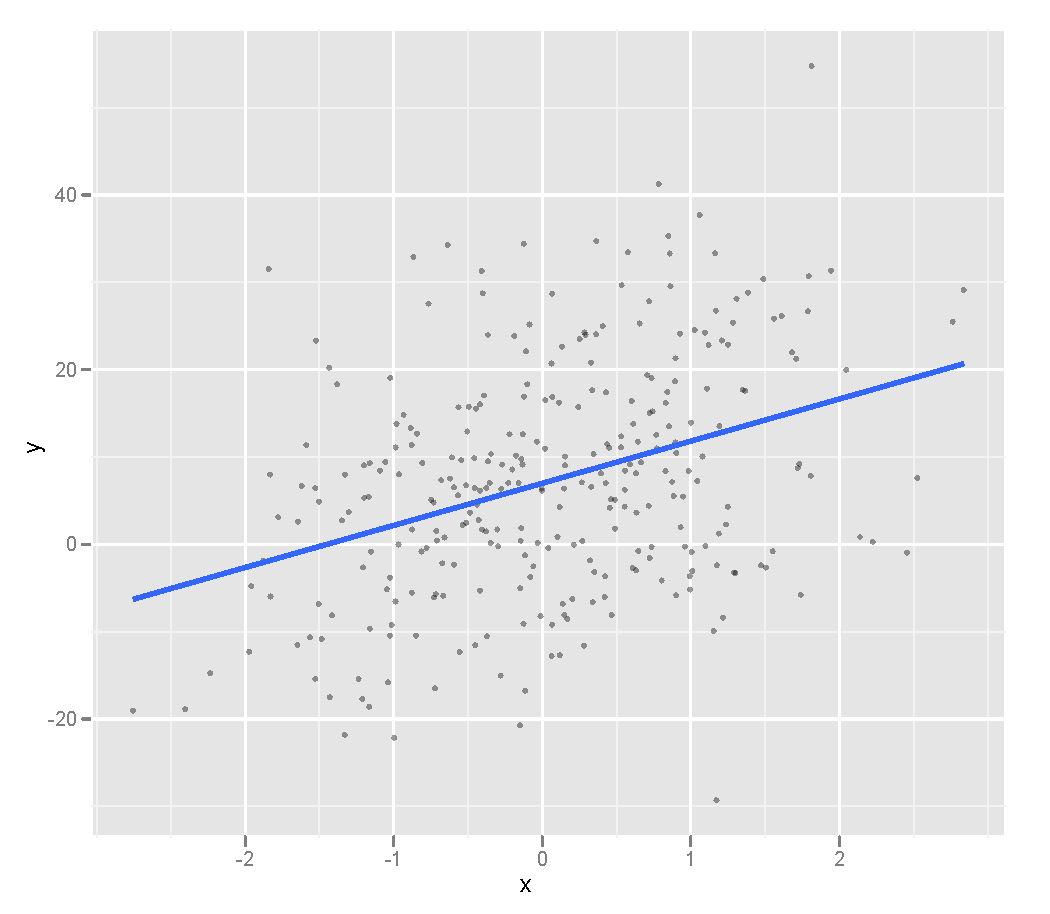
\includegraphics{scatter_plot_beta_4.pdf}}
       \caption{Scatter plot of data generated for $\beta_0$=6, $\beta_1$=4, sample size $n =300$ and $\sigma = 12$. $R^2$ for this data was obtained as 0.1309 showing that the model could not successfully explain the variation in $Y$. But notice in figure \ref{fig:power_rsq} that power for $\beta$=4 is almost 1. So, Can we conclude that $R^2$ does not have any effect in deciding whether $H_0: \beta_1=0$ should be rejected or not?}
       \label{fig:plot_beta_4}
\end{figure}


\begin{figure}[hbtp]
   \centering
       \scalebox{.35}{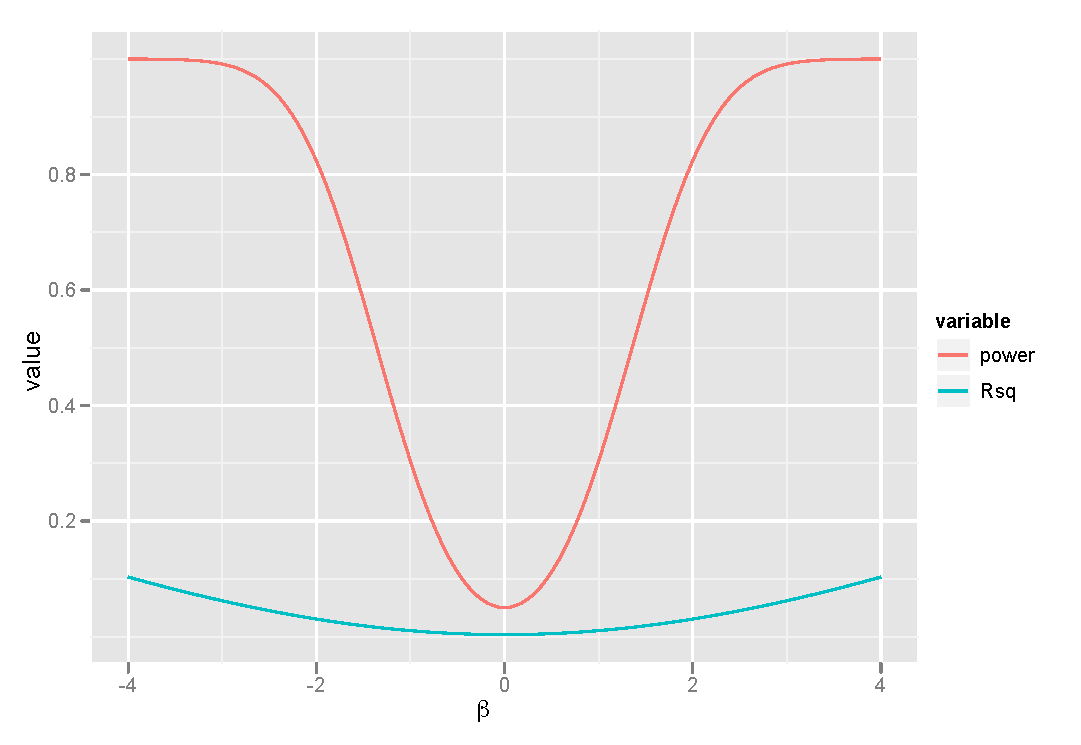
\includegraphics{power_300_12.pdf}}
       \caption{Power curve and $R^2$ values for sample size $n =300$ and $\sigma = 12$. Notice that for a small value of $R^2$ (0.1) the power is almost 1.}
       \label{fig:power_rsq}
\end{figure}


\begin{figure}[hbtp]
   \centering
       \scalebox{.35}{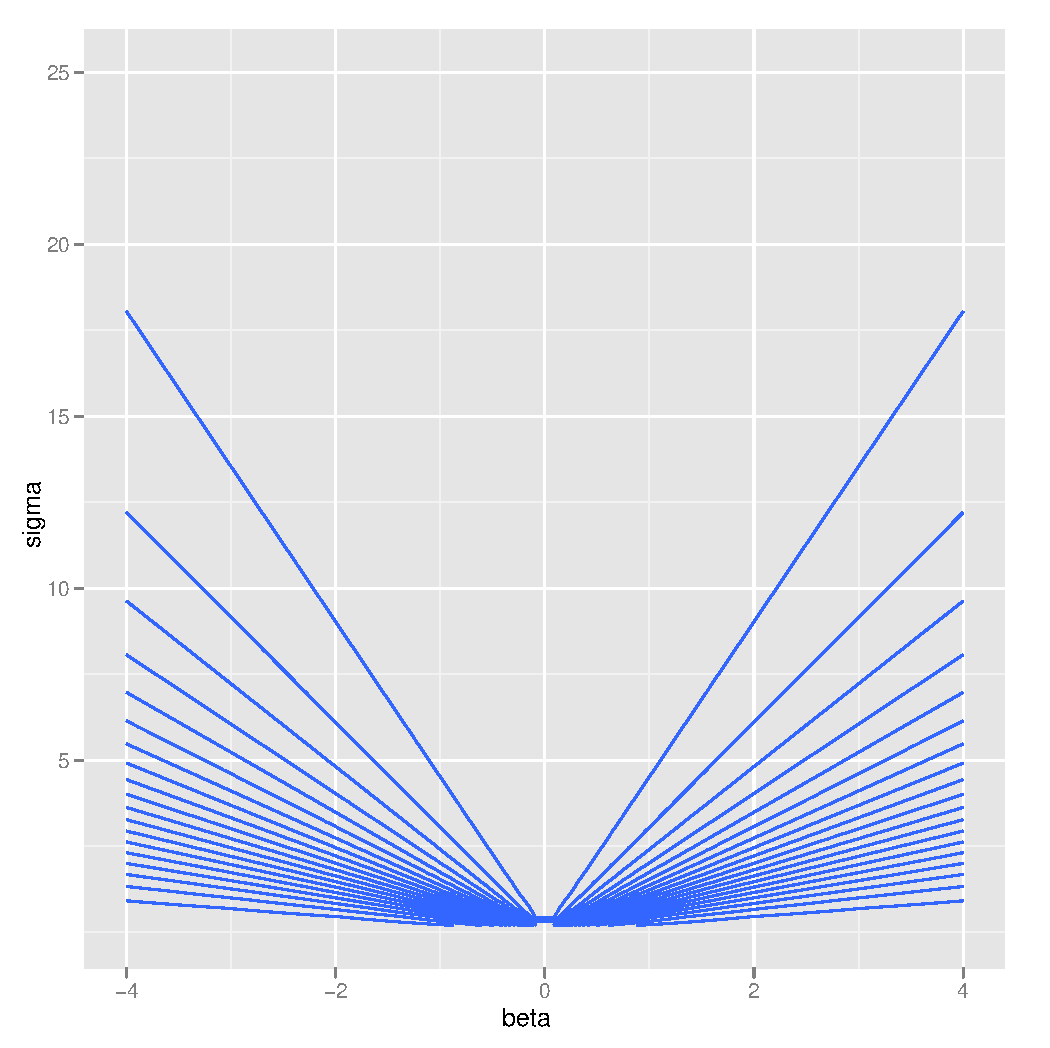
\includegraphics{rsquare_contour.pdf}}
       \scalebox{.35}{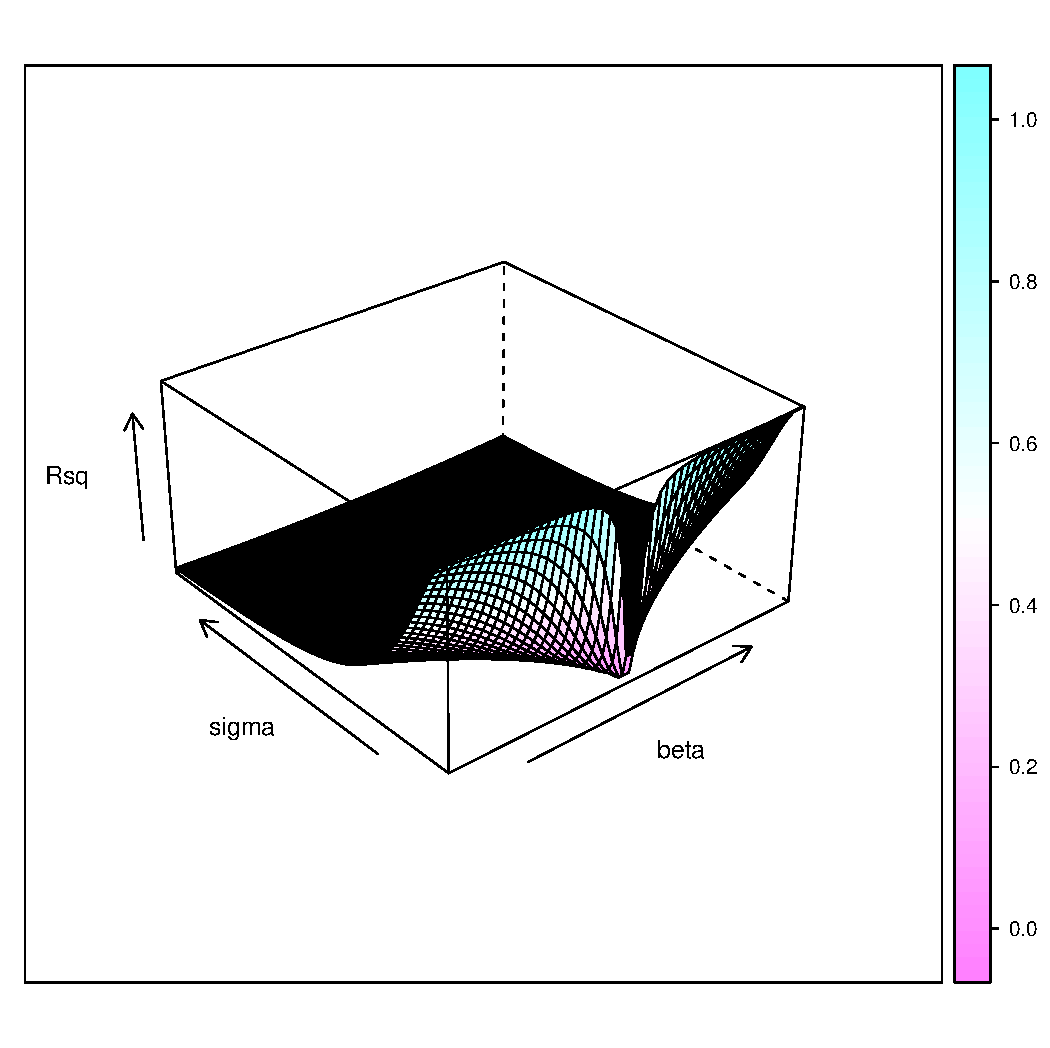
\includegraphics{rsquare_beta_sigma.pdf}}
       \caption{Contour and surface plots of $R^2$ for sample size $n =300$. The values for $R^2$ goes down sharply with $\sigma$ and $\beta$.}
       \label{fig:contour_rsq}
\end{figure}

\begin{figure}[hbtp]
   \centering
       \scalebox{.35}{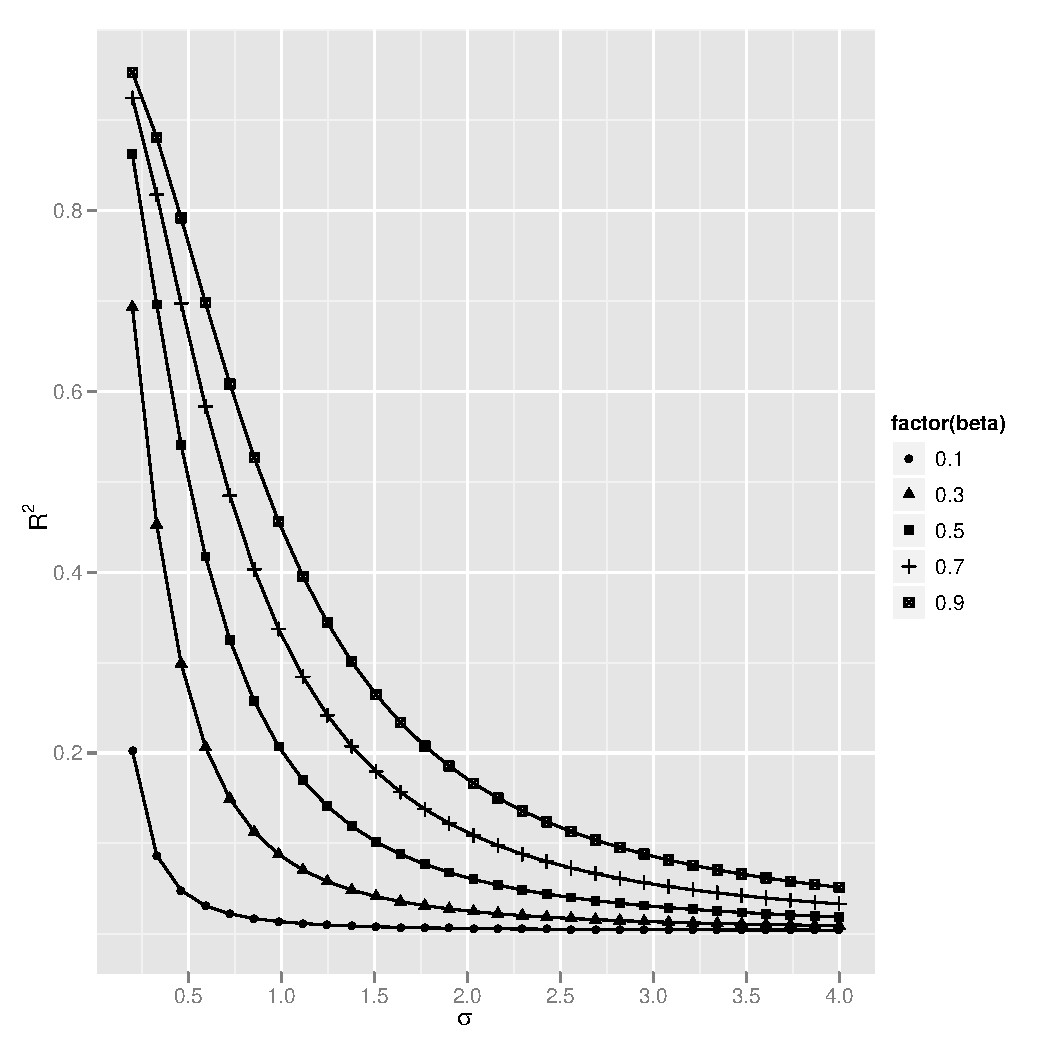
\includegraphics{rsquare_beta_sigma_lines.pdf}}
       \scalebox{.35}{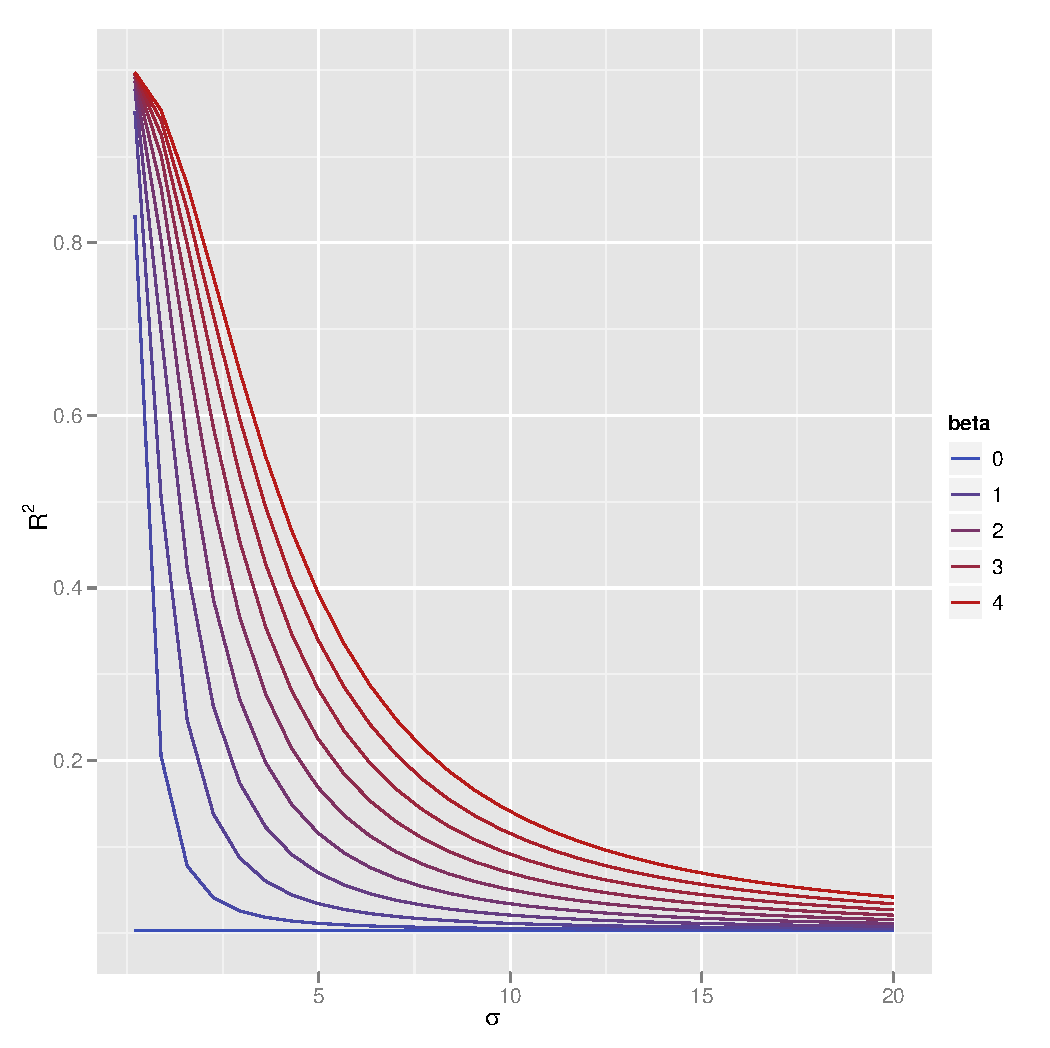
\includegraphics{rsquare_beta_sigma_lines1.pdf}}       
       \caption{Relationship of $R^2$ with $\sigma$ and $\beta$ for sample size $n =300$. The values for $R^2$ goes down sharply with $\sigma$ and $\beta$.}
       \label{fig:rsq}
\end{figure}




\bibliographystyle{plain}
\bibliography{references} 

\end{document}


